\documentclass{article}

\usepackage{amsmath}
\usepackage{amsfonts}
\usepackage{amssymb}
\usepackage{graphicx}
\usepackage{hanging}

\usepackage[letterpaper, margin=1in]{geometry}

\usepackage{algorithm}

\usepackage{multicol, color}
\usepackage[noend]{algpseudocode}
\newcommand*\Let[2]{\State #1 $\gets$ #2}
\algrenewcommand\algorithmicrequire{\textbf{Precondition:}}
\algrenewcommand\algorithmicensure{\textbf{Postcondition:}}

\newcommand{\todo}{\textcolor{red}}

\newenvironment{proof}[1][Proof]{\textbf{#1.} }{\ \rule{0.5em}{0.5em}}
\newtheorem{theorem}{Theorem}
\newtheorem{lemma}{Lemma}

% Document starts
\begin{document}
	
	% Title portion
	\title{Money maketh men: An examination of order book algorithms}
	\author{Sophiya Chiang and Serena Fan}
	
\date{\today}

\maketitle

\begin{abstract}
This paper aims to study order matching algorithms, which dictate how trades are executed and therefore offer crucial insight into the operation of securities exchanges. We begin with a brief history of financial markets to establish the context of trades. Then, we delve into some relevant definitions and concepts to properly define the problem of order matching. Next, we focus on the two most common techniques in trade allocation, namely FIFO matching and pro-rata matching algorithms, and discuss their properties and potential impacts on the market. The analyses from this paper give us a basic overview of how trade orders are matched via algorithms in an exchange.
\end{abstract}

\section{Introduction}

The financial industry offers many interesting algorithmic problems that command our modern economy. Market forces are driven by trades and nearly all  trading activity operates within clearly defined structures. We hope to learn more about the techniques that dictate the majority of our trading activity in order to understand how computer science plays a major stake in finance. We will zero in on order matching and two of its most commonly used algorithms.

The first trade occurred in Amsterdam when the Dutch East India Company introduced easily transferable shares in 1602. By 1680, the general public was engaging in a multitude of complex trades, including forwards, futures, and options. The computerization of order flow began in the 1970s, and notable innovation was the NYSE's "designated order turnaround" system which sent orders electronically and executed them manually. The SEC later officially authorized electronic exchanges in 1998. It also ordered all U.S. stock markets to convert to decimalization from the current fractional system. This caused the minimum price difference to fall from 0.0625 USD (1/16th) to 0.01 USD. The SEC's actions served as a catalyst for the rise of high frequency trading (HFT) because it allowed for a tighter spread (smaller disparities between bid and offer prices), thus decreasing the market makers’ trading advantage and increasing market liquidity. By 2012, HFT trades had reached an execution time of mere nanoseconds. These trades have not only made gains in speed, but are also accounting for an increasingly larger fraction of all equity orders: only 10 percent of all equity trades in the U.S. were made by HFT in 2001. By 2012, this rose to 70 percent. Our decision to focus on order matching algorithms was derived from its ability to provide a good introduction into the incredibly relevant world of HFT and that it is relatively easy to understand.


\section{Order matching problem}
 
The problem we are discussing is known by myriad of names including "order book matching", "trade allocation", or "trade matching", but the problem itself is the process of executing a trade in an order book. 

In the following sections, we will delve into some formal definitions that pertain to order matching so as to provide sufficient context. We will then present a formal description of the algorithms we are focusing on and compare and contrast their properties.  

\subsection{Order matching}
Order matching refers to the mechanism of pairing off buy orders and sell orders to execute securities trades. There are different types of orders an investor can place in an exchange and each type dictates how the orders are fulfilled in an exchange. Some of the different types include, but are not limited to, market orders, limit orders, and stop-loss orders. Each of these have their own set of rules that could potentially maximize the investor's profits and minimize potential loss. Understanding the different order types can help us understand when to use certain type of order matching algorithms. For simplicity's sake, let us consider market orders and limit orders. \\\\
\textbf{Market orders:} Market orders are the easiest way to buy or sell a stock. Orders placed by investors are filled as quickly as possible at best available current price, with no time or price limitations. A wide bid-ask spread may result from these orders since investors want these trades to go through in minimal time.\\\\
\textbf{Limit orders:} A limit order is an order that specifies the price for a purchase or sale regardless of the time it takes to execute the order. A buy limit order is an order to purchase a security at or below a specified price, such that traders can specify the price they are willing to pay to purchase a security, also known as the bid price. This guarantees that the investor pays the specified price or better in a trade. Whereas, a sell limit order specifies a price, the asking price, that will only be executed at the limit price or higher.\\\\
To successfully execute a trade, exchanges utilize various matching algorithms to determine the price and quantity at which an order is filled. Stock prices on electronic exchanges are determined at each tick by a matching algorithm which matches buyers with sellers, who can be thought of as independent agents engaged in an “acceptable” price negotiation or a continuous double auction.

\subsection{Order book} 
Order books are lists maintained by the exchange of the buy and sell orders for specific securities or financial instruments submitted by market participants. At any given moment, the order book is recording the prices and quantities of a given security the traders are willing to buy or sell at in order to create a continuous book keeping. Information in the order book allow investors to make informed trading decisions. ********Depending on the product and matching priority of the exchange, order books can be implemented by various different data structures. \todo{not sure if i should add this part but i want to because its more computer science-y but more details might be needed}******** 

\subsection{Matching principles: A problem description}
When the market is open, traders are constantly submitting their buy or sell orders; this mechanism can be thought of as a continuous double auction in order to achieve the fairest price.\\\\
Different exchanges use various ways of matching the orders in the order book depending on the types of securities traded or the type of orders placed. We have chosen two different techniques that are often used in the exchanges, specifically FIFO and pro-rata order matching, both of which are online algorithms in practice as they continuously depend on market conditions at different points in time.\\\\
When orders are entered into the electronic order book, they are sorted by type, price, and submission time. For matching purposes, market orders are given the highest priority. FIFO matching, also known as price-time priority matching, is a technique often used in exchanged traded products while pro-rata matching is often used for money market products with smaller intraday price fluctuations.\\\\
\textbf{FIFO matching. } With FIFO matching, an order is entered with a time-stamp associated with it. The time-stamp is down to the millisecond and prioritizes the orders in the order book with the same price. The order that was entered earliest at a given price gets executed first. This grouping of trades with the same price occurs continuously throughout the trading day.\\\\
\textbf{Pro-rata matching. } Meanwhile, pro-rata matching is usually used with products that have low intraday bid-ask price volatility. When a new order is entered into the trading system, the algorithm searches the order book and executes matching orders in proportion to the orders already contained in the order book, by taking into account every book order at the best bid or ask price according to its percentage of the overall volume that is bid or offered at the given price. The time-stamp of an order is ignored and therefore the algorithm ensures constant access for orders of all sizes.\\\\

The multiple price levels in a limit order book can be modeled as a multi-class queuing network.???? \todo{elaborate on this if we add it, might need to add more on data structures} \\
	\begin{figure}[h]
		\centering
		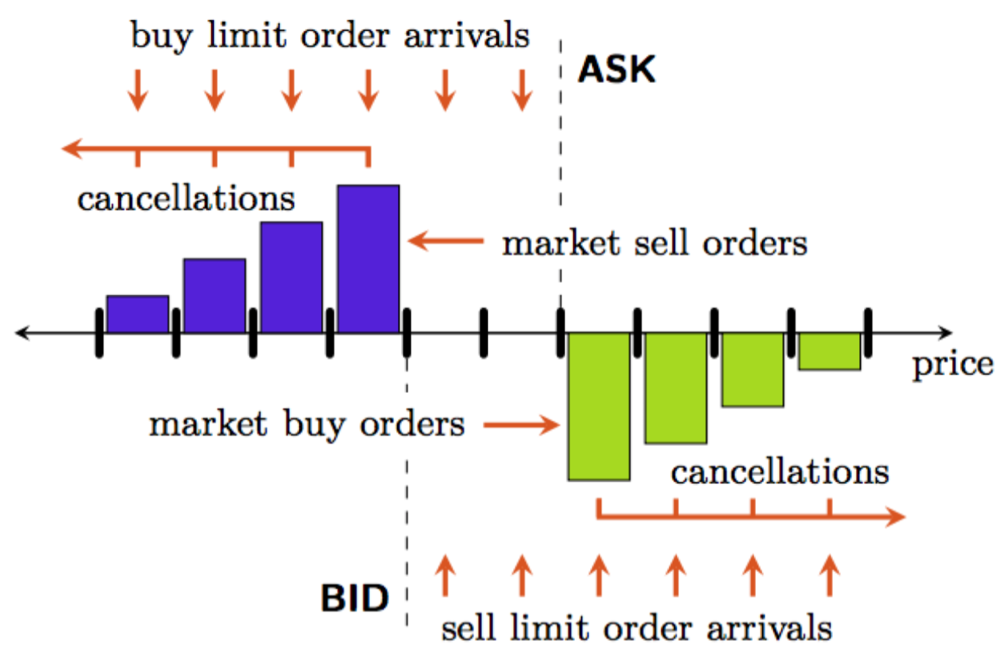
\includegraphics[width=0.5\linewidth]{chart.png}
		\caption{https://pdfs.semanticscholar.org/40be/6b083e5cc502e0ddcb1335b040822237a09a.pdf}
		\label{fig}
	\end{figure}

\todo{do we want more diagrams? or none at all?}

\section{Overview of algorithms}
The following section highlights the two most commonly employed algorithms for order matching, namely the FIFO  algorithm and the pro-rata algorithm. These two algorithms match orders based on different mechanisms, and we will provide a comparison of the two approaches after discussing their respective strategies in detail.

\subsection{FIFO algorithm}
Using the first-in, first-out method (FIFO), an incoming trade is paired with the first orders at the best price.
Consider an incoming market order of $N$ lots (the number of lots indicates the minimum traded volume of the market order) such that $N\leq Q$, where $Q$ indicates the cumulative volume of existing orders. Suppose that this market order is traded against $n$ limit orders such that $Q_1... Q_n$ make up the total volume of $Q$ lots. Then, there exists an index $j$ such that $1\geq j \geq n$, such that,
\begin{center}
    $\sum_{i=1}^j Q_i \leq N$, and\\
    $\sum_{i=1}^{min(j+1, n)} Q_i \geq N$
\end{center}
are fulfilled. The FIFO algorithm will thus fill the first j limit orders in full and assign the remaining lots to the $(j + 1)th$ limit order if $j < n$.

\subsection{Pro-rata algorithm}
Instead of by time priority, an  incoming trade is divided among limit orders in proportion to their sizes. Consider the same incoming market order of $N$ lots traded against $n$ limit orders of $Q_1\ldots Q_n$ for a total volume $Q$ lots, such that $N \leq Q$.\\\\
Each order $Q_i$ has a pro-rata proportion $p_i $ that helps determine the number of lots that it receives. This proportion is determined by a simple calculation as shown below. $\forall$ order $i < n$, 
\begin{center}
    $p_i = \dfrac{Q_i}{Q}$
\end{center}
The number of lots obtained by an order $Q_i$ is found by multiplying the pro-rata proportion with the total number of lots in the market order, 
\begin{center}
    $Q_i = floor(p_i * N)$.
\end{center}
 The remaining lots can be redistributed in many ways, one of the most common being FIFO, as defined above with price/time. Another option is to designate one lot for each unfilled order, and assign remaining lots to the orders that have a pro-rata proportion $p_i < 1$ in descending $p_i$ value, thus providing extra incentive for small market players. 

\subsection{A comparison of the algorithms}
The two algorithms have very distinct applications because of their differences. FIFO algorithms deter the addition of new orders because these orders will have last priority in the queue. On the other hand, pro-rata orders encourage new orders to join the queue with large limit orders because the total quoted volume at the best price will be large too. FIFO algorithms also have the potential for larger complexity because market players are more inclined to flood the market by placing limit orders in the “depth of the market” to stay in the queue. However, this algorithm is able to naturally narrow the spread since the limit order becomes first in the queue when the spread is narrowed. Pro-rata algorithms do not share this feature, which is a notable disadvantage. FIFO algorithms are more frequently used while pro-rata algorithms are great for specific applications including derivative contracts with many expirations. 

\subsection{Analysis}
There is a distinct lack of available real data in current research on matching algorithms due to the secrecy of the trading industry. Thus, authors of academic papers in this area generally rely on virtual simulations instead of real experiments. The nature of order matching algorithms themselves also make analyzing their complexities difficult as they are online algorithms.

\section{Discussion and summary}
Understanding the order matching algorithms used in various exchanges is an important step to developing trade strategies. The two algorithms described in this paper are but the tip of the iceberg; there are a plethora of order book matching algorithms out there and due to their proprietary nature, it is difficult to find scholarly sources on trade secrets.\\\\
Since the field of computational finance combines the study of mathematics, statistics, finance, and computer science, most of our research extend beyond the scope of this paper. Also, most academic journals focus on simulations of actual market conditions  and it is difficult to find relevant research that focuses on pure computer science theory. Thus, though we can theoretically postulate how these algorithms work, it is often difficult to simulate the real trading behaviors on any given day.\\\\

\newpage

% Bibliography
\bibliographystyle{abbrv}
\bibliography{bibfile}                

\begin{hangparas}{.25in}{1}

Works Cited
\\ 

AG, Eurex Frankfurt. “Navigation.” Eurex Exchange - What Actually Is pro Rata Matching?, 24 Aug. 2015.

Anderson, Erik. “Adaptive Strategies for High Frequency Trading.” JOURNAL OF STELLAR MS&E, 2008.

Bonart, Julius, and Martin D. Gould. “Latency and Liquidity Provision in a Limit Order Book.” Quantitative Finance, vol. 17, no. 10, Oct. 2017, pp. 1601–1616., doi:10.1080/14697688.2017.1296177.

Carrel, Lawrence. “Understanding Different Buy and Sell Orders When Managing Stocks.” Dummies.

“History of Algorithmic Trading, HFT and News Based Trading.” Evolution of Algorithmic Trading, HFT and News Based Trading, 12 Dec. 2016.

“History of Algorithmic Trading, HFT and News Based Trading.” Evolution of Algorithmic Trading, HFT and News Based Trading, 12 Dec. 2016.

Janeˇcek, Karel, and Martin Kabrhel. Matching Algorithms of International Exchanges. 1 Dec. 2007.

Preis, Tobias. Price-Time Priority and Pro Rata Matching in an Order Book Model of Financial Markets.

Staff, Investopedia. “Matching Orders.” Investopedia, 23 Nov. 2003.

Staff, Investopedia. “Order Book.” Investopedia, 2 Oct. 2013.
\end{hangparas}

\newpage

Documentation of edits \\
\todo{figure out how to restart numbering or just put on a separate document}

\section{Introduction}
\begin{itemize}

  \item Condensed the introduction as we spent too long on this portion during the Monday presentations, deleted unnecessary explanations and definitions
  
\end{itemize}
\section{Order matching problem}
\begin{itemize}

  \item Put this portion into own words and then restructured the organization 
  
\end{itemize}
\section{Overview of algorithms}
\begin{itemize}

  \item Simplified the explanation of pro-rata algorithms as a student did not understand it during the Monday presentations.
  
\end{itemize}
\section{Discussion and summary}
\begin{itemize} 

  \item Put more context around the conclusion as context of the algorithm was naturally explained  during the Monday presentations so people would understand the lack of available analysis
  
\end{itemize}
\end{document}